\documentclass[12pt]{article}

% Настройка русского языка и шрифтов
\usepackage[utf8]{inputenc}
\usepackage[russian]{babel}
\usepackage[T2A]{fontenc}

% Математические пакеты
\usepackage{amsmath, amssymb, amsfonts}

% Настройка страницы
\usepackage{geometry}
\geometry{a4paper, margin=0.8in}

% Другие полезные пакеты
\usepackage{hyperref}
\usepackage{booktabs}
\usepackage{enumitem}
\usepackage{longtable}
\usepackage{graphicx}
\usepackage{xcolor}

% Определение стилей для комментариев
\definecolor{commentgray}{rgb}{0.4,0.4,0.4}
\definecolor{antigravityblue}{rgb}{0.0, 0.45, 0.74}

\newcommand{\commentary}[1]{{\small\itshape\color{commentgray} #1}}
\newcommand{\antigravity}[1]{{\small\color{antigravityblue}\textbf{Antigravity:} #1}}

% Настройка ссылок
\hypersetup{
    colorlinks=true,
    linkcolor=blue,
    filecolor=magenta,      
    urlcolor=cyan,
    pdftitle={Глубокий разбор: Метрики качества},
}

\title{Глубокий разбор: Метрики классификации и регрессии}
\author{Твой персональный гид по ML}
\date{\today}

\begin{document}

\section{Типология метрик}

\subsection{Офлайновые метрики}
Офлайновые метрики вычисляются на исторических данных (тестовых выборках) без участия реальных пользователей.

\begin{itemize}
    \item \textbf{Зачем нужны}: 
    \begin{itemize}
        \item Для быстрой итерации и сравнения моделей между собой.
        \item Для отбора лучших кандидатов перед запуском дорогостоящих A/B-тестов.
        \item Для отладки алгоритма и поиска его слабых мест (анализ ошибок).
    \end{itemize}
    \item \textbf{Примеры}: Accuracy, Precision, Recall, ROC-AUC, RMSE, MAE.
\end{itemize}

\subsection{Онлайновые метрики}
Онлайновые метрики измеряются в реальном времени при взаимодействии системы с «живыми» пользователями в ходе A/B-тестирования.

\begin{itemize}
    \item \textbf{Зачем нужны}: 
    \begin{itemize}
        \item Для оценки реального влияния модели на бизнес-показатели.
        \item Для учета поведенческих факторов и внешних эффектов (например, сезонность или действия конкурентов).
        \item Для проверки «прокси-гипотез» (коррелирует ли рост ROC-AUC с ростом выручки).
    \end{itemize}
    \item \textbf{Примеры}: CTR (Click-Through Rate), Конверсия (CR), ARPU (Average Revenue Per User), время сессии, Retention.
\end{itemize}

\subsection{Ключевые отличия}
\begin{longtable}{@{}lll@{}}
\toprule
\textbf{Характеристика} & \textbf{Офлайн} & \textbf{Онлайн} \\ \midrule
Источник данных & Исторические данные & Реальные пользователи \\
Скорость получения & Минуты/часы & Дни/недели \\
Стоимость & Дешево (CPU/GPU) & Дорого (риск потери прибыли) \\
Объективность & Оценивает модель & Оценивает продукт/бизнес \\ \bottomrule
\end{longtable}

\commentary{Главная проблема ML в продакшене — отсутствие корреляции между офлайн и онлайн метриками. Модель может идеально предсказывать вероятность клика (высокий ROC-AUC), но показывать плохой CTR из-за того, что предлагаемые товары неинтересны пользователям в данный момент.}

\section{Функция потерь vs Метрика качества}

Часто новички путают эти понятия, так как в некоторых задачах (например, в регрессии) они могут совпадать (MSE). Однако это концептуально разные вещи.

\subsection{Функция потерь (Loss Function)}
Это математический инструмент для \textbf{обучения} модели.
\begin{itemize}
    \item \textbf{За что отвечает}: Показывает, насколько сильно модель «ошиблась» на конкретном объекте или выборке.
    \item \textbf{Как используется}: Минимизируется градиентными методами (SGD, Adam) для настройки весов.
    \item \textbf{Требования}: Должна быть \textbf{дифференцируемой} (или иметь субградиент), чтобы мы могли вычислить производную.
    \item \textbf{Примеры}: LogLoss, Cross-Entropy, Huber Loss.
\end{itemize}

\subsection{Метрика качества (Metric)}
Это инструмент для \textbf{оценки} модели человеком или бизнесом.
\begin{itemize}
    \item \textbf{За что отвечает}: Показывает реальное качество работы модели в понятных единицах (проценты, рубли, количество ошибок).
    \item \textbf{Как используется}: Для принятия решения о запуске модели, сравнения алгоритмов, мониторинга.
    \item \textbf{Требования}: Должна быть \textbf{интерпретируемой}. Не обязана быть дифференцируемой.
    \item \textbf{Примеры}: Accuracy, F1-score, ROC-AUC.
\end{itemize}

\subsection{В чем ключевые отличия?}
\begin{enumerate}
    \item \textbf{Цель}: Loss — для оптимизатора, Metric — для человека.
    \item \textbf{Гладкость}: Функция потерь должна быть гладкой. Метрика может быть дискретной (например, Accuracy меняется скачками).
    \item \textbf{Интерпретируемость}: Мы редко можем сказать, что означает «LogLoss = 0.23» в терминах бизнеса, но «Accuracy = 95\%» понятно всем.
\end{enumerate}

\commentary{Почему нельзя просто минимизировать Accuracy? Потому что её производная везде равна нулю (или не существует), и градиентный спуск не сможет сдвинуть веса модели с места. Поэтому мы используем LogLoss как «дифференцируемый суррогат» для Accuracy.}



\section{Матрица ошибок (Confusion Matrix)}

Матрица ошибок — это таблица, позволяющая визуализировать производительность алгоритма классификации.

\begin{table}[h]
\centering
\begin{tabular}{lcc}
\toprule
& \textbf{Y=1 (Positive)} & \textbf{Y=0 (Negative)} \\
\midrule
\textbf{a(x)=1} & TP (True Positive) & FP (False Positive) \\
\textbf{a(x)=0} & FN (False Negative) & TN (True Negative) \\
\bottomrule
\end{tabular}
\caption{Матрица ошибок для бинарной классификации.}
\end{table}

\begin{figure}[h]
	\centering
	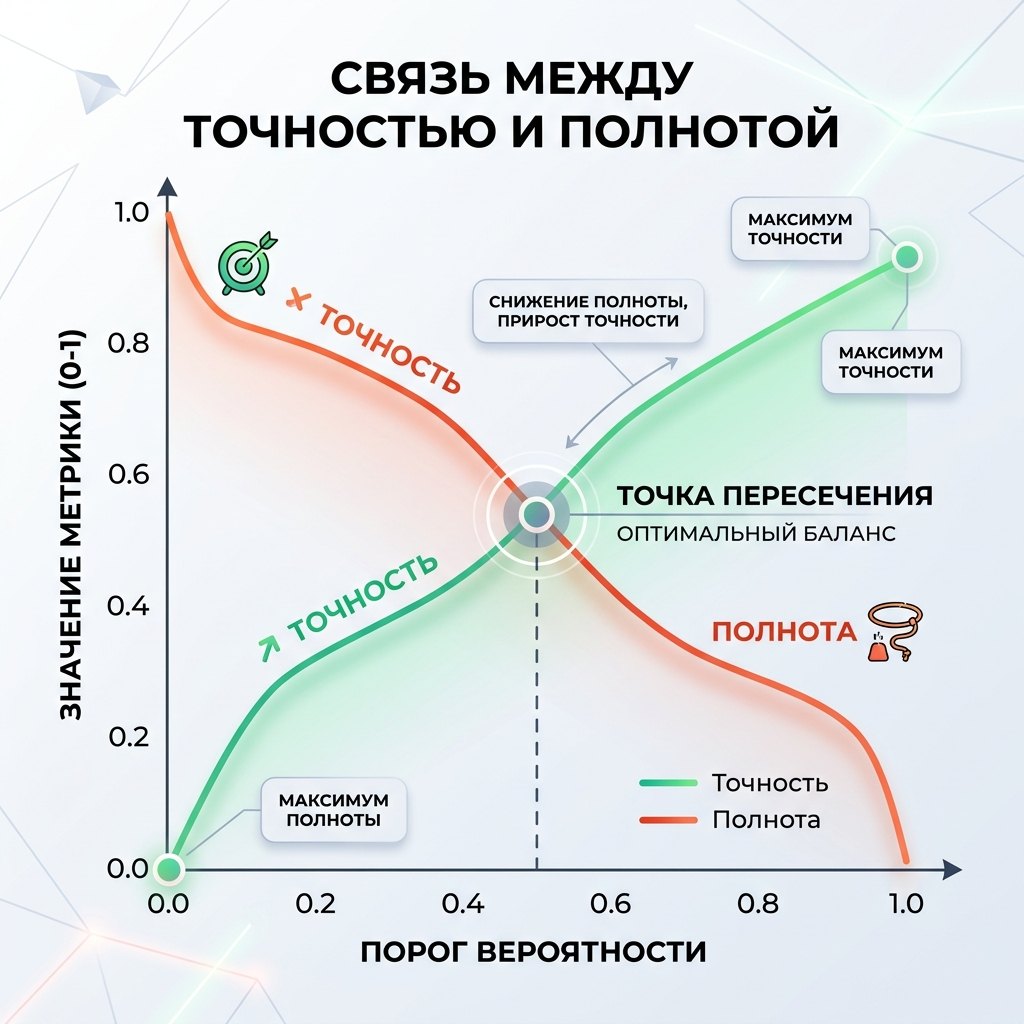
\includegraphics[width=0.6\textwidth]{pr_tradeoff.png}
	\caption{Компромисс между точностью и полнотой.}
\end{figure}

\subsection{Основные метрики качества}

На основе матрицы ошибок вычисляются базовые метрики:

\begin{itemize}
    \item \textbf{Accuracy} (Доля правильных ответов): Показывает общую точность модели.
    \[ \text{Accuracy} = \frac{TP + TN}{TP + TN + FP + FN} \]
    
    \item \textbf{Precision} (Точность): Доля истинно положительных среди всех объектов, которые алгоритм отнес к положительному классу. Помогает минимизировать количество ложных срабатываний (FP).
    \[ \text{Precision} = \frac{TP}{TP + FP} \]
    
    \item \textbf{Recall} (Полнота): Доля истинно положительных среди всех объектов положительного класса. Помогает минимизировать количество пропусков (FN).
    \[ \text{Recall} = \frac{TP}{TP + FN} \]
    
    \item \textbf{F1-measure} (F-мера): Гармоническое среднее между точностью и полнотой. Позволяет оценить модель одним числом, когда важны и Precision, и Recall.
    \[ F_1 = 2 \cdot \frac{\text{Precision} \cdot \text{Recall}}{\text{Precision} + \text{Recall}} = \frac{2 \cdot TP}{2 \cdot TP + FP + FN} \]
\end{itemize}

\commentary{Precision и Recall часто находятся в противофазе: пытаясь улучшить одну метрику, мы обычно ухудшаем другую. Выбор баланса между ними зависит от цены ошибки (что хуже: ложная тревога или пропуск цели?).}

\begin{longtable}{lp{0.35\textwidth}p{0.35\textwidth}}
	\toprule
	\textbf{Метрика} & \textbf{Пример задачи} & \textbf{Где ЗАПРЕЩЕНО} \\
	\midrule
	Accuracy & Распознавание цифр & Фрод (сильный дисбаланс) \\
	Precision & Таргетинг (высокая цена звонка) & Поиск пропавших (важен каждый сигнал) \\
	Recall & Диагностика рака (нельзя пропустить) & Спам-фильтр (важные письма не в спам) \\
	F1-measure & Поиск в базе знаний & Когда Recall критичнее Precision \\
	\bottomrule
\end{longtable}

\begin{figure}[h]
    \centering
    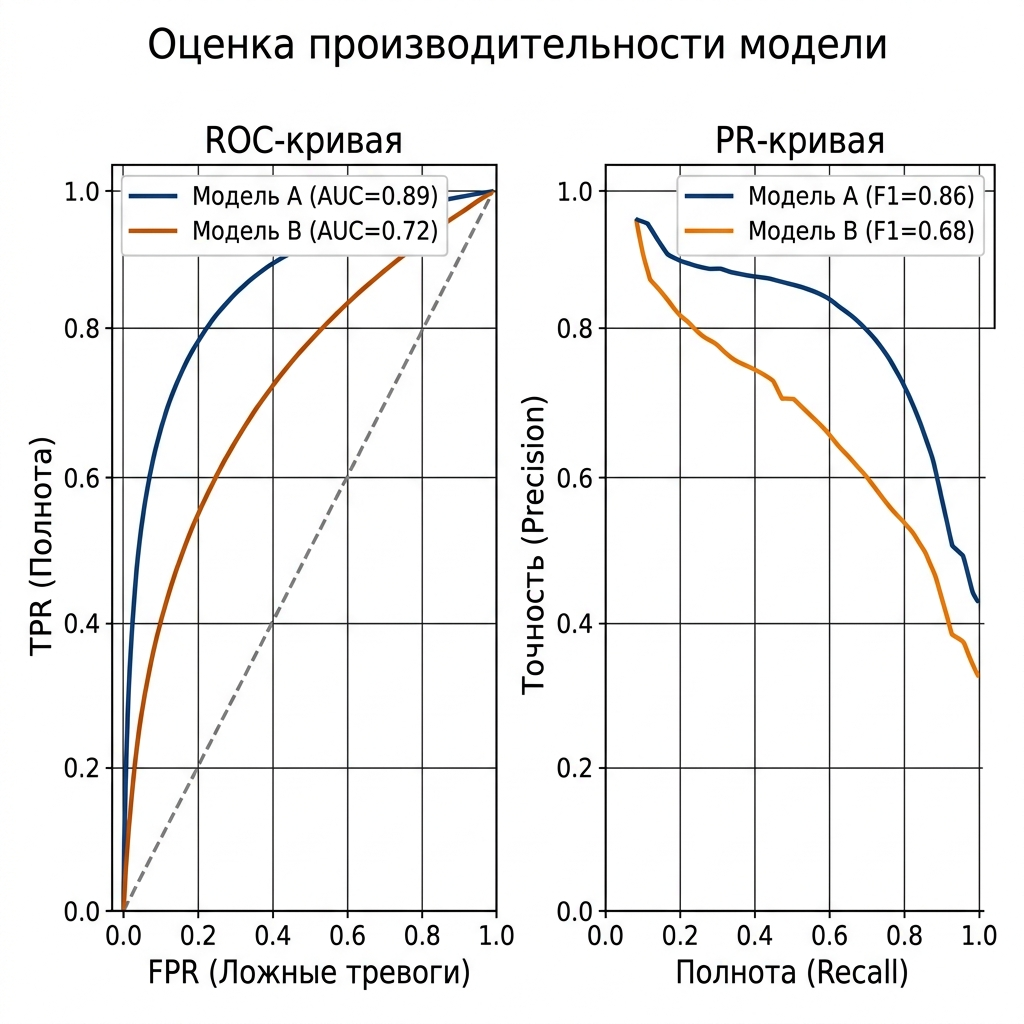
\includegraphics[width=0.5\textwidth]{roc_vs_pr.png}
    \caption{Сравнение ROC и PR кривых.}
\end{figure}

\section{Кривые и площади: ROC-AUC и PR-AUC}

Эти метрики оценивают качество **ранжирования** объектов моделью, а не просто точность предсказания классов при фиксированном пороге.

\subsection{ROC-AUC (Receiver Operating Characteristic)}
Кривая строится в осях:
\begin{itemize}
    \item \textbf{TPR} (True Positive Rate / Recall): $\frac{TP}{TP + FN}$.
    \item \textbf{FPR} (False Positive Rate): $\frac{FP}{FP + TN}$.
\end{itemize}

\textbf{Суть}: Показывает долю пар объектов разного класса, которые алгоритм верно упорядочил (положительный объект имеет оценку выше отрицательного).

\begin{itemize}
    \item \textbf{Плюсы}: 
    \begin{itemize}
        \item Не зависит от порога классификации.
        \item Устойчива к изменению баланса классов (формулы TPR и FPR нормируются внутри своего класса).
    \end{itemize}
    \item \textbf{Минусы}: 
    \begin{itemize}
        \item На сильно несбалансированных данных (например, 1:1000) может быть обманчиво высокой, даже если модель ошибается на большинстве реальных позитивных объектов.
    \end{itemize}
    \item \textbf{Где подходит}: Задачи с более-менее сбалансированными классами.
\end{itemize}

\subsection{PR-AUC (Precision-Recall Curve)}
Кривая строится в осях:
\begin{itemize}
    \item \textbf{Recall} (Полнота).
    \item \textbf{Precision} (Точность).
\end{itemize}

\begin{itemize}
    \item \textbf{Плюсы}: 
    \begin{itemize}
        \item Явно фокусируется на качестве предсказания редкого (положительного) класса.
        \item Очень чувствительна к ложным срабатываниям (FP), что критично для задач с дисбалансом.
    \end{itemize}
    \item \textbf{Минусы}: 
    \begin{itemize}
        \item Сильно зависит от баланса классов в обучающей выборке. При изменении доли позитивных объектов кривая «просядет» или поднимется.
    \end{itemize}
    \item \textbf{Где подходит}: Задачи с сильным дисбалансом (фрод, дефектоскопия, редкие заболевания).
\end{itemize}


\commentary{Главное правило: если классы сбалансированы — смотри на ROC-AUC. Если есть сильный дисбаланс — PR-AUC даст гораздо более честную картину.}


\section{Метрики регрессии}

В задачах регрессии мы предсказываем вещественное число $\widehat{y} \in \mathbb{R}$.

\subsection{MSE (Mean Squared Error)}
Среднеквадратичная ошибка.
\[ MSE = \frac{1}{n} \sum_{i=1}^n (y_i - \widehat{y}_i)^2 \]
\begin{itemize}
    \item \textbf{Плюсы}: Хорошая «математика» (выпуклая, дифференцируемая), сильно штрафует за большие отклонения.
    \item \textbf{Минусы}: Неустойчива к выбросам (один выброс может «утянуть» значение метрики), трудно интерпретировать (единицы измерения в квадрате).
\end{itemize}

\subsection{MAE (Mean Absolute Error)}
Средняя абсолютная ошибка.
\[ MAE = \frac{1}{n} \sum_{i=1}^n |y_i - \widehat{y}_i| \]
\begin{itemize}
    \item \textbf{Плюсы}: Устойчива к выбросам (робастна), легко интерпретируется (единицы измерения совпадают с таргетом).
    \item \textbf{Минусы}: Не дифференцируема в нуле (сложнее использовать как Loss).
\end{itemize}

\begin{figure}[h]
    \centering
    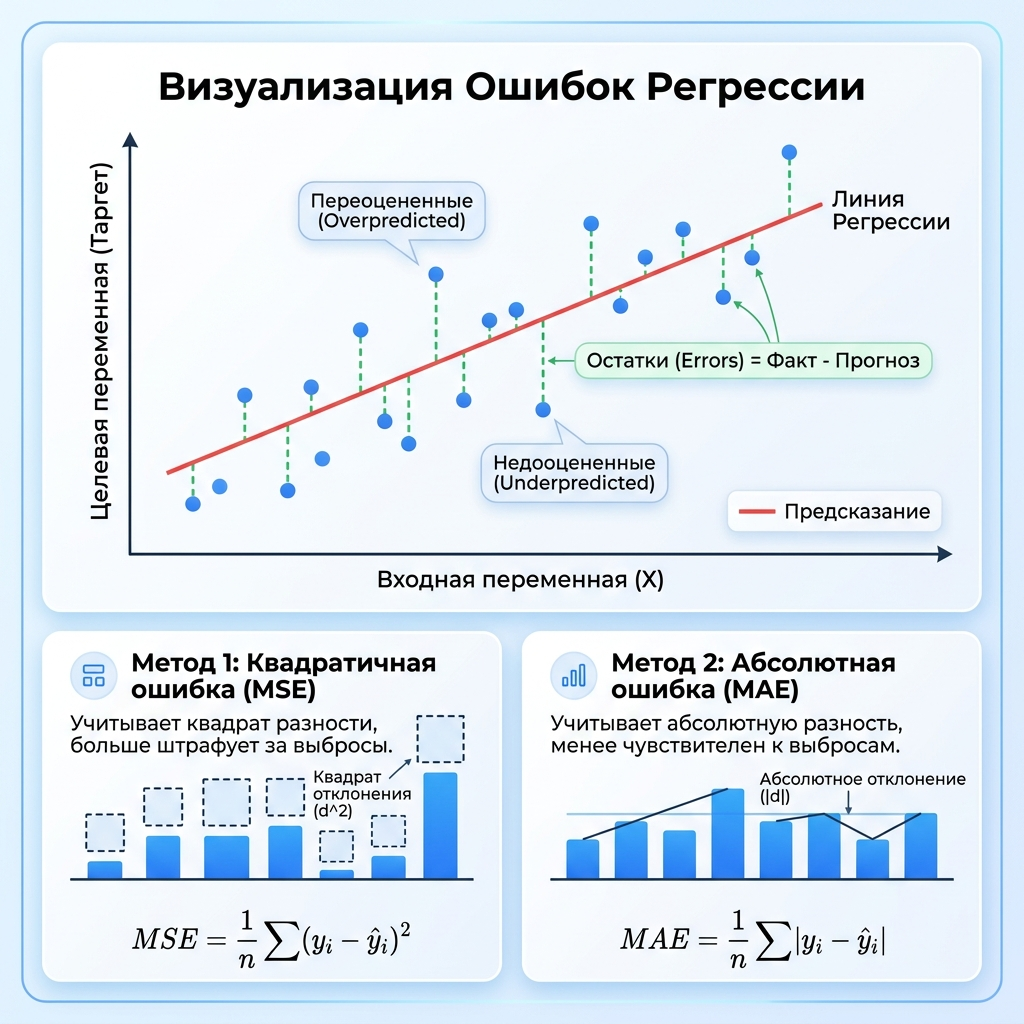
\includegraphics[width=0.6\textwidth]{regression_errors.png}
    \caption{Визуализация: MSE (слева) гораздо сильнее реагирует на выбросы, чем MAE (справа).}
\end{figure}

\subsection{Относительные метрики: MAPE, SMAPE, WAPE}
Используются, когда нам важна не абсолютная ошибка, а ошибка в процентах от величины таргета.

\begin{itemize}
    \item \textbf{MAPE} (Mean Absolute Percentage Error):
    \[ MAPE = \frac{100\%}{n} \sum_{i=1}^n \left| \frac{y_i - \widehat{y}_i}{y_i} \right| \]
    \commentary{Плохо: нельзя использовать, если в данных есть нули ($y_i=0$). Асимметрична: сильнее штрафует за занижение прогноза, чем за завышение.}
    
    \item \textbf{SMAPE} (Symmetric MAPE):
    \[ SMAPE = \frac{100\%}{n} \sum_{i=1}^n \frac{|y_i - \widehat{y}_i|}{(|y_i| + |\widehat{y}_i|)/2} \]
    \commentary{Решает проблему деления на ноль (если $\widehat{y}_i$ не ноль) и уменьшает асимметрию.}
    
    \item \textbf{WAPE} (Weighted MAPE):
    \[ WAPE = \frac{\sum_{i=1}^n |y_i - \widehat{y}_i|}{\sum_{i=1}^n |y_i|} \]
    \commentary{Позволяет избежать проблем с околонулевыми значениями отдельных объектов, суммируя ошибки по всей выборке.}
\end{itemize}

\subsection{RMSLE (Root Mean Squared Logarithmic Error)}
\[ RMSLE = \sqrt{\frac{1}{n} \sum_{i=1}^n (\log(y_i + 1) - \log(\widehat{y}_i + 1))^2} \]
\begin{itemize}
    \item \textbf{Зачем}: Когда таргет меняется на порядки (цены на жилье, продажи). Штрафует за относительную ошибку, а не абсолютную.
    \item \textbf{Особенность}: Сильнее штрафует за **занижение** прогноза ($y > \widehat{y}$), чем за завышение.
\end{itemize}

\antigravity{Метрики — это мост между бизнесом и математикой. Неверный выбор метрики ведет к созданию идеальной, но бесполезной модели.}

\end{document}
